%% LyX 2.0.6 created this file.  For more info, see http://www.lyx.org/.
%% Do not edit unless you really know what you are doing.
\documentclass[]{paper}
\usepackage{fontspec}
\setmainfont[Mapping=tex-text]{华文仿宋}
\setsansfont[Mapping=tex-text]{华文细黑}
\setmonofont{华文细黑}
\usepackage{listings}
\usepackage{graphicx}
\makeatletter
\usepackage{xeCJK}
\makeatother

\usepackage{xunicode}
\usepackage{polyglossia}
\setdefaultlanguage{}
\begin{document}

\title{ 连续曲线的优化问题}
\author{徐浩}

\maketitle
\begin{abstract}

\end{abstract}


\section{问题}
求解$\vec{x}(t)$,使得
$$\delta \int_a^b f(\vec x)dt=0$$
\subsection{解空间}
空间中的所有曲线
\subsection{解}
最优曲线

\subsection{思路}

\begin{enumerate}
\item 雪崩
\item 水流
\item  元胞自动机
\end{enumerate}
如何归纳这些问题的共性。
\section{空间离散化与SPFA}
哈密顿原理是经典力学的重要原理。在传统应用中,哈密顿原理主要通过对Ldt积分的变分来实践中应用,又或者通过费马原理在光学问题中应用,鲜有直接使用的方法。而我们适用计算机的最短路算法,将空间离散化,重新定义了空间中的范数(在微分情况下)。根据范数定义,在离散后的非欧空间内使用SPFA最短路算法得出最短路径(在简单问题中,可以认为其变分为零),也就是位形空间内的解。\\
SPFA需要对于空间的离散化,我采用了随机点生成并且使用kd树进行临近点查找的算法生成大量网格。然后对生成路径附近撒点,进行再次细化。迭代数次。\\
高维条件下的情况还在优化中。。。\\
这个算法对于非完全约束有一定优势(比如变分法无论如何都无法一次得到有障碍物的捷线,我们可以简单给出)\\
对于捷线问题,我是这么做的
\begin{quotation}
空间中比较接近的两点(由收敛半径确定)
距离定义为
$$\frac{ds}{\sqrt y}$$
也就是 $$dist(0,1)=\sqrt{\frac{   (x_0-x_1)^2+(y_0-y_1)^2}{y}} $$
这样子的话,每一条路径就是$\frac{dv}{v}$的求和,当曲线细分时,就是$$T=\int_0^1 \frac{ds}{v} $$
\end{quotation}

算法是先生成50000随机点,产生一条路径,在路径上以路径临界两点画正方形,在此正方形内随机产生共5w点。然后迭代6-7次。可以得到一条紧密的曲线。然后mathematica插值之。可以得到结论。

下面是一个收敛算法产生的图形
蓝色,黄色,灰色,粉红,绿色点分别表示每一次随机产生的点,黑色则是最后的轨道,插值输出的。
\begin{center}
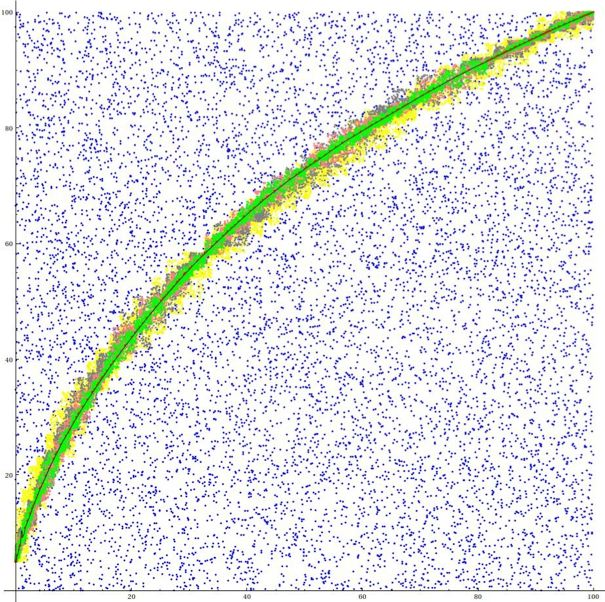
\includegraphics[width=1\linewidth]{./spfa0}
\end{center}
单列的图
\begin{center}
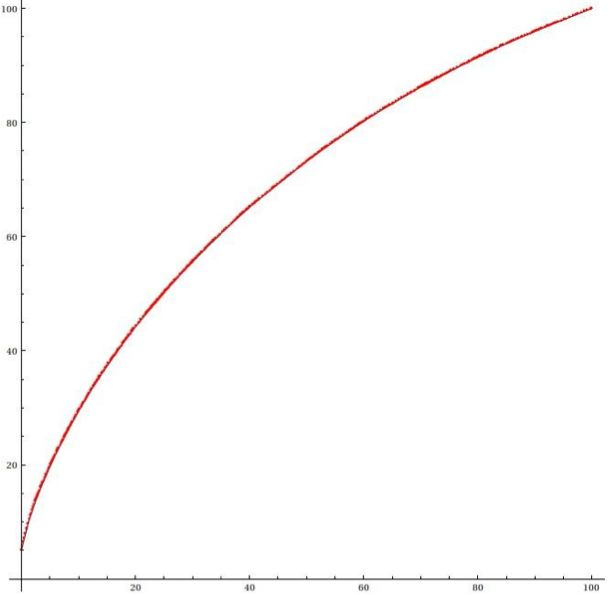
\includegraphics[width=1\linewidth]{./spfa1}
\end{center}
\section{一些分析} 
上面这个算法是去年做的,当时也用来做了电磁学论文,在这里不再赘述.\\

其缺点在于因为对于空间进行了细分,所以时间,空间复杂度会随着维数的上升而极度上升,毫无应用价值可言.但是其思想在于通过全局最优解来获得力学问题的全部状态信息还是有其用武之地.\\

在最近的思考中,我想到,既然我们可以将力学问题归纳成泛函问题,那么为什么不能将泛函问题再次转化为力学问题呢\\

在洗澡的时候,水流引起了我的注意,根据张力定理,一个水流的总的表面积应当是最小的.那么水流很容易可以获得一个曲面上的最短路径.我将水流的流动剖析为以下几个性质
\begin{enumerate}
\item 首先是水流会因为自身的张力而发生收缩,其性质类似于弹簧振子在阻尼情况下的区域能量最低态,
\item 其二是水流相遇的时候会因为张力而发生汇流,合成一股新的水流,合并过程中遵循质心定理.
\item 再有是水流的产生符合随机行走过程.
\end{enumerate}

我们试想一个哭泣的女孩(其实是某日晚上我想好这个算法的时候后睡前想某同学,就无意中脑补脸上流出水流),其第一滴泪和前面的眼泪会因为毛孔,空气等原因方向各异,我们无妨称之为"涕泗横流".然而大哭后面的眼泪终究会因为重力的拖拽而走出一条合适的路径(假设该同学哭泣时候仍然保持自习时的标准坐姿).这条路径之于女孩的面容应当基本符合$$\delta
 \int_a^b f(\vec x)dt=0$$
也就是说,假设重力成为了时间,女孩的脸成为了相空间(y-y'),那么我们就得到了某一个量在相空间的泛函.
\section{张力水流}
\subsection{Assumption}

再无引力的情况下,我们认为水流会趋向于合并到表面积最小的状况.符合物理原理,最小能量原理。再有,对于泛函问题,空间中局部最优解也是合格的解.因为局部最优解总是符合变分为零.所以我们的曲线要么发散,要么收敛,但凡收敛,都是系统在相空间内可能的运行路径.
\subsection{定理}

合并定理\\

松弛定理\\

随机行走(对解空间的遍历)\\
\subsection{产生方法}
随机行走\\
步长与当前f相关.\\
\subsection{合并方法}
拉链式合并
\subsection{n+1维空间中蜷曲的n维曲面上求解最短路之松弛定理}
\begin{center}
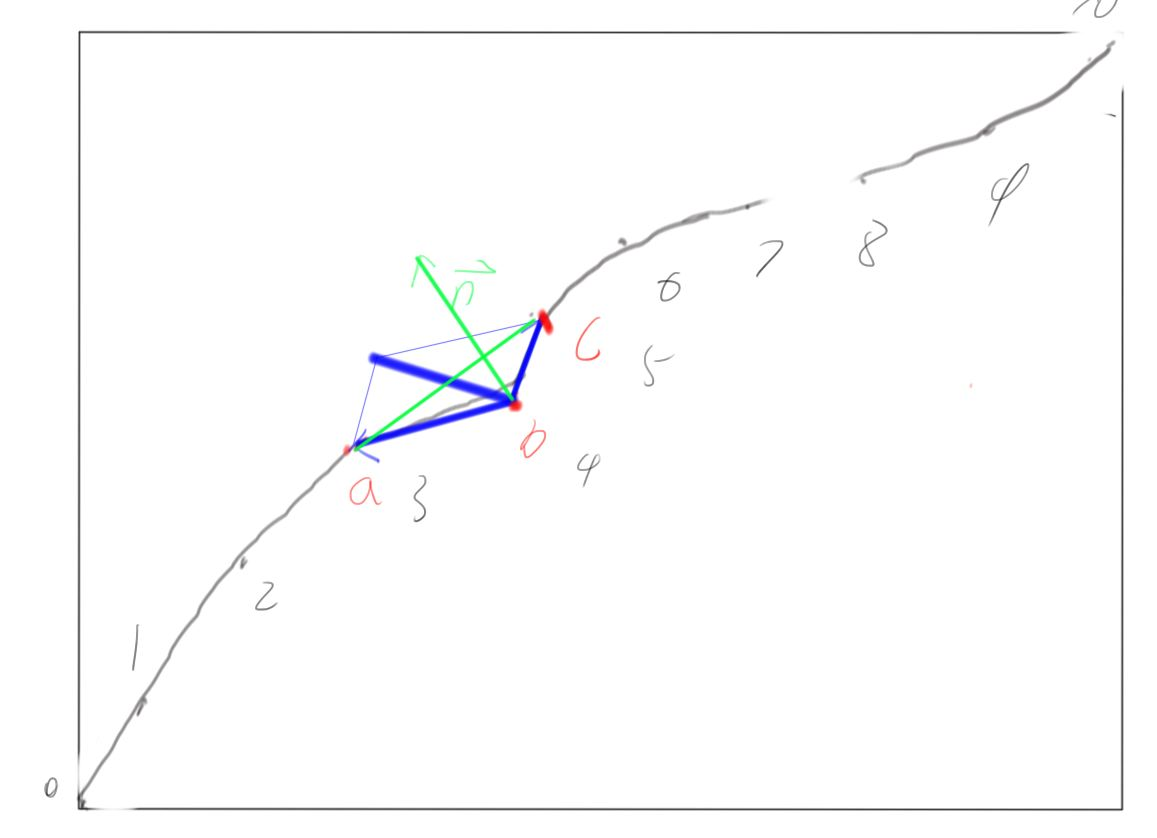
\includegraphics[width=1\linewidth]{./Image001}
\end{center}
在处理松弛问题的时候,曲线上的每一个点更像是一组弹簧上的质点,点和点之间的互相作用正比与距离,同时我们认为每次点的运动距离正比与其力的大小.并且为边长所限制.\\
其基本定理是,
\begin{quotation}
 对于一系列弹簧振子,其平衡位置是其能量最低点.亦即,全局长度最短的状态.
\end{quotation}
那么有,千万不要忘记支持力!!$\vec N$,也就是去掉$\vec F$在$\vec n$上面的分量
\begin{eqnarray}
&&\vec{ac}=(c_x-a_x,c_y-a_y)\\
&&\vec n=(-f'_x(x,y),-f'_y(x,y),1)\\
&&\vec F_p=\frac{(x_i-x_{i-1},y_i-y_{i-1},z_i-z_{i-1})}{\sqrt{\Delta x^2+\Delta y^2+\Delta z^2}}\\
&&\vec F_n=\frac{(x_{i+1}-x_{i},y_{i+1}-y_{i},z_{i+1}-z_{i})}{\sqrt{\Delta x^2+\Delta y^2+\Delta z^2}}\\
&&\vec F_{tens}=\vec F_n+\vec F_p\\
&&\Sigma \vec F=\vec F_{tens}+\vec N
\end{eqnarray}
其中支持力$\vec N$
有 $$\vec N=-(\vec F_{tens}\cdot \vec n)\vec n\\$$
那么,
\begin{eqnarray} 
&&\Sigma \vec F=\vec F_{tens}+\vec N\\
&&\Delta q_b=\alpha \Sigma \vec F
\end{eqnarray}

  如此松弛迭代,得到了能量最低的弹簧组的构型即是所求n+1维空间中n维曲面上A点到B点最短路.\\

  这个方法的巧妙之在于,随着空间维数的增加,我们求解问题规模的数量级并不发生改变.
 \subsection{转化}
 下面的问题是如何将泛函问题转化为一个距离问题.\\
 
 首先我们要霸气侧漏的重新定义空间范数(距离),令$g(x,y)$并不显含时间
 $$Norm (a,b)=\int_b^a g(\vec x(t)) dt $$
 其中$x(t)$使得
$$\delta \int_a^b g(\vec x)dt=0$$
于是我们得到了一个全新的非欧空间,在这个空间内任意两点间距离是其最小泛函的值.\\

泰勒展开,在a和b点非常接近的情况下
$$\int_a^b g(\vec x(t))dt=\lim_{b\rightarrow a}g(\vec x(t))\cdot (t_b 
-t_a)+\frac{g'_{\vec b-\vec a}(\vec x(t))\cdot (t_b -t_a)}{2}$$
于是我们可以得到微观下的距离定义.从而将距离定义带入到前面的松弛法中,获得泛函问题的解答.
\subsection{优点}
只用链表完成对空间中曲线的遍历
\section{雪崩或者河流的迁移}
引力牵引,合并沟槽,类似与三峡。
\section{元胞自动机?}


\end{document}
